\section{Partie 3 : Réseau de neurones}
    \subsection{IA : Généralités}
        \begin{frame}[allowframebreaks]{IA : Généralités}
            \begin{block}{Généralités}
                \begin{itemize}
                    \setbeamertemplate{itemize item}[square]
                    \item Détection d'anomalies :
                        \begin{itemize}
                            \item Absence de tube sur la palette
                            \item Absence de bouchon sur la palette
                        \end{itemize}
                    \item Calcul sur serveur :
                        \begin{itemize}
                            \item VM Linux 4C/8T alloué et 50Go de RAM
                            \item Nvidia Quadro P4000
                            \item Intel Xeon Gold 5122 à 3.6GHz
                        \end{itemize}
                \end{itemize}
            \end{block}
            
            \begin{block}{Réseau de neurone utilisé : YoloV5}
                \begin{itemize}
                    \setbeamertemplate{itemize item}[square]
                    \item Réseau neuronal profond
                    \item Prise en main très rapide
                    \item Rapide à mettre en place
                    \item Système de détection d'objets temps réel (vidéos, images)
                \end{itemize}
            \end{block}
           
        \end{frame}
%
% ---------------------------------------------------------------- %
    \subsection{IA : LabelImg}
        \begin{frame}[allowframebreaks]{IA : LabelImg}
            \begin{columns}
                \begin{column}{0.5\textwidth}
                    \begin{block}{LabelImg}
                        \begin{itemize}
            	            \setbeamertemplate{itemize item}[square]
            	            \item Logiciel libre (disponible sur GitHub)
            	            \item Écrit en python
            	            \item Sert pour \textbf{\underline{Yolo}} \& PascalVOC
            	            \item Ecrit un fichier texte sous forme : \textit{classe centreX centreY largeur hauteur}
            	        \end{itemize}
                    \end{block}
                \end{column}\hfill
                \begin{column}{0.5\textwidth}
                    \begin{figure}[H]
                        \centering
                        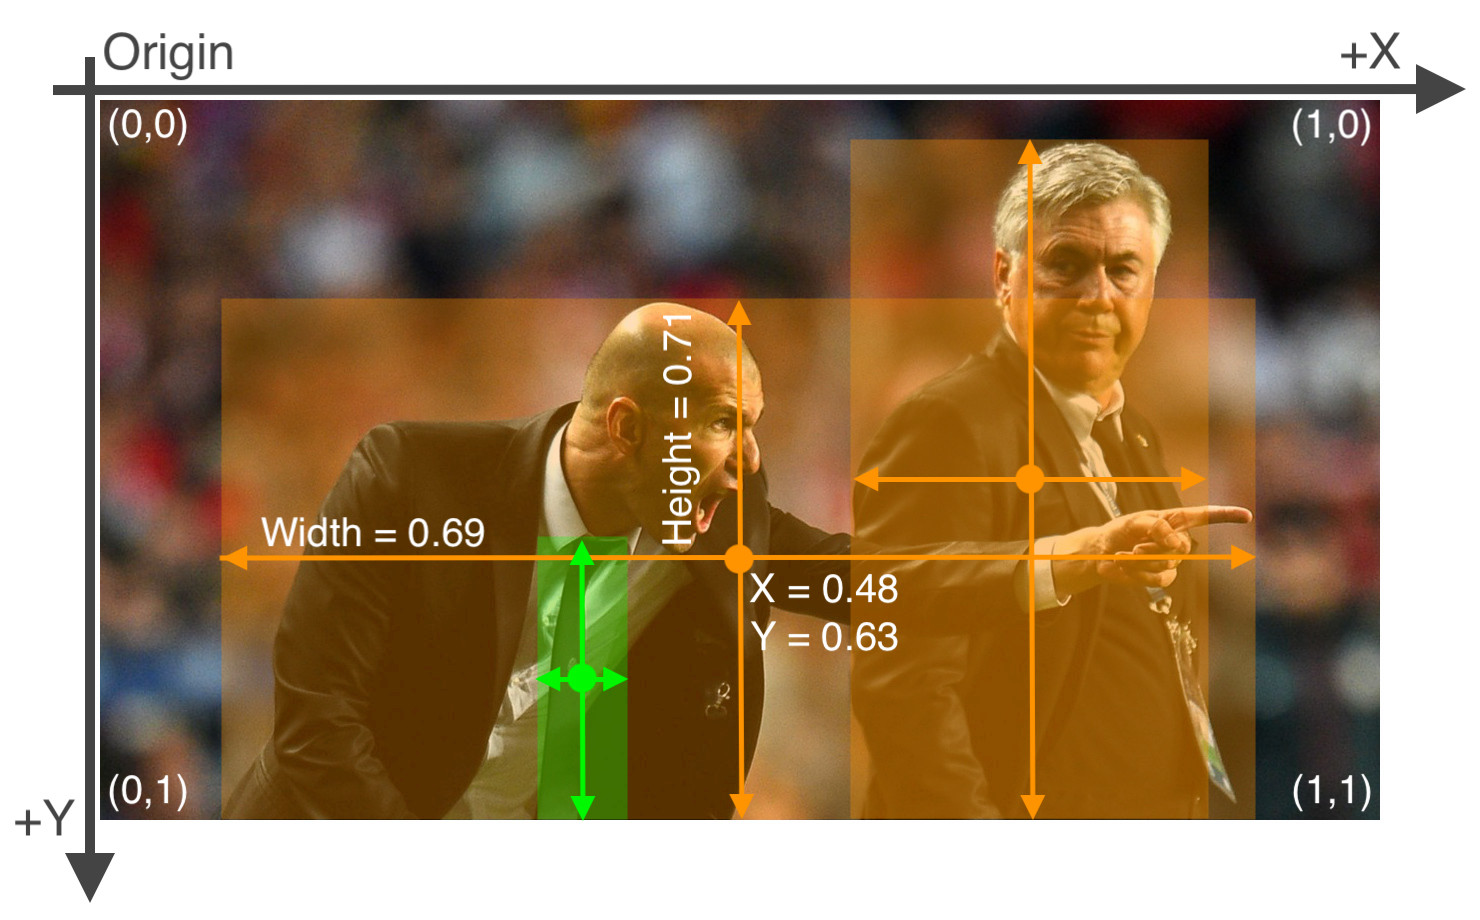
\includegraphics[width=1\linewidth]{images/exempleImgYolo.png}
                    \end{figure}
                \end{column}
            \end{columns}
            
            \begin{figure}[H]
                \centering
                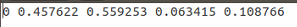
\includegraphics[width=1\linewidth]{images/labelTxt.png}
            \end{figure}
            
            %\begin{figure}[H]
             %   \centering
            %    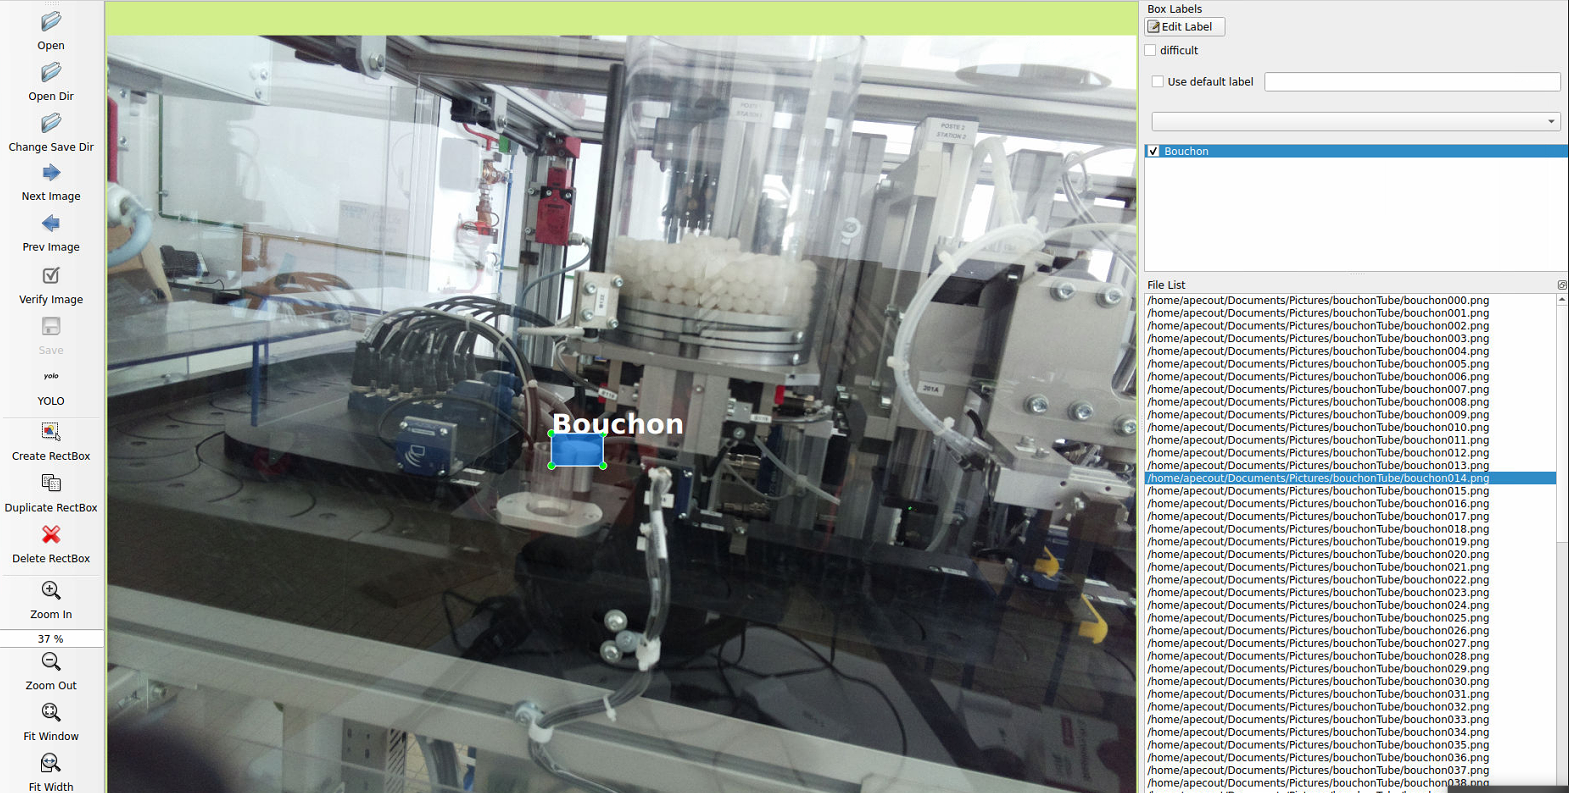
\includegraphics[width=1\linewidth]{images/uiLabelImg.png}
            %\end{figure}
        \end{frame}
%
% ---------------------------------------------------------------- %
    \subsection{IA : YoloV5}
        \begin{frame}[allowframebreaks]{IA : YoloV5}
            %\begin{columns}
             %   \begin{column}{0.4\textwidth}
             %       \begin{block}{}
             %           \begin{itemize}
            %	            \setbeamertemplate{itemize item}[square]
            %	            \item $FP_{16}$ : représente Float Point 16
            %	            \item Nvidia Tesla V100 - moyenne sur 5000 images
            %	            \item mAP : mean Average Precision (moyenne des précisions moyennes)
            %	        \end{itemize}
            %        \end{block}
            %    \end{column}\hfill
            %    \begin{column}{0.6\textwidth}
            %        \begin{figure}[H]
            %            \centering
            %            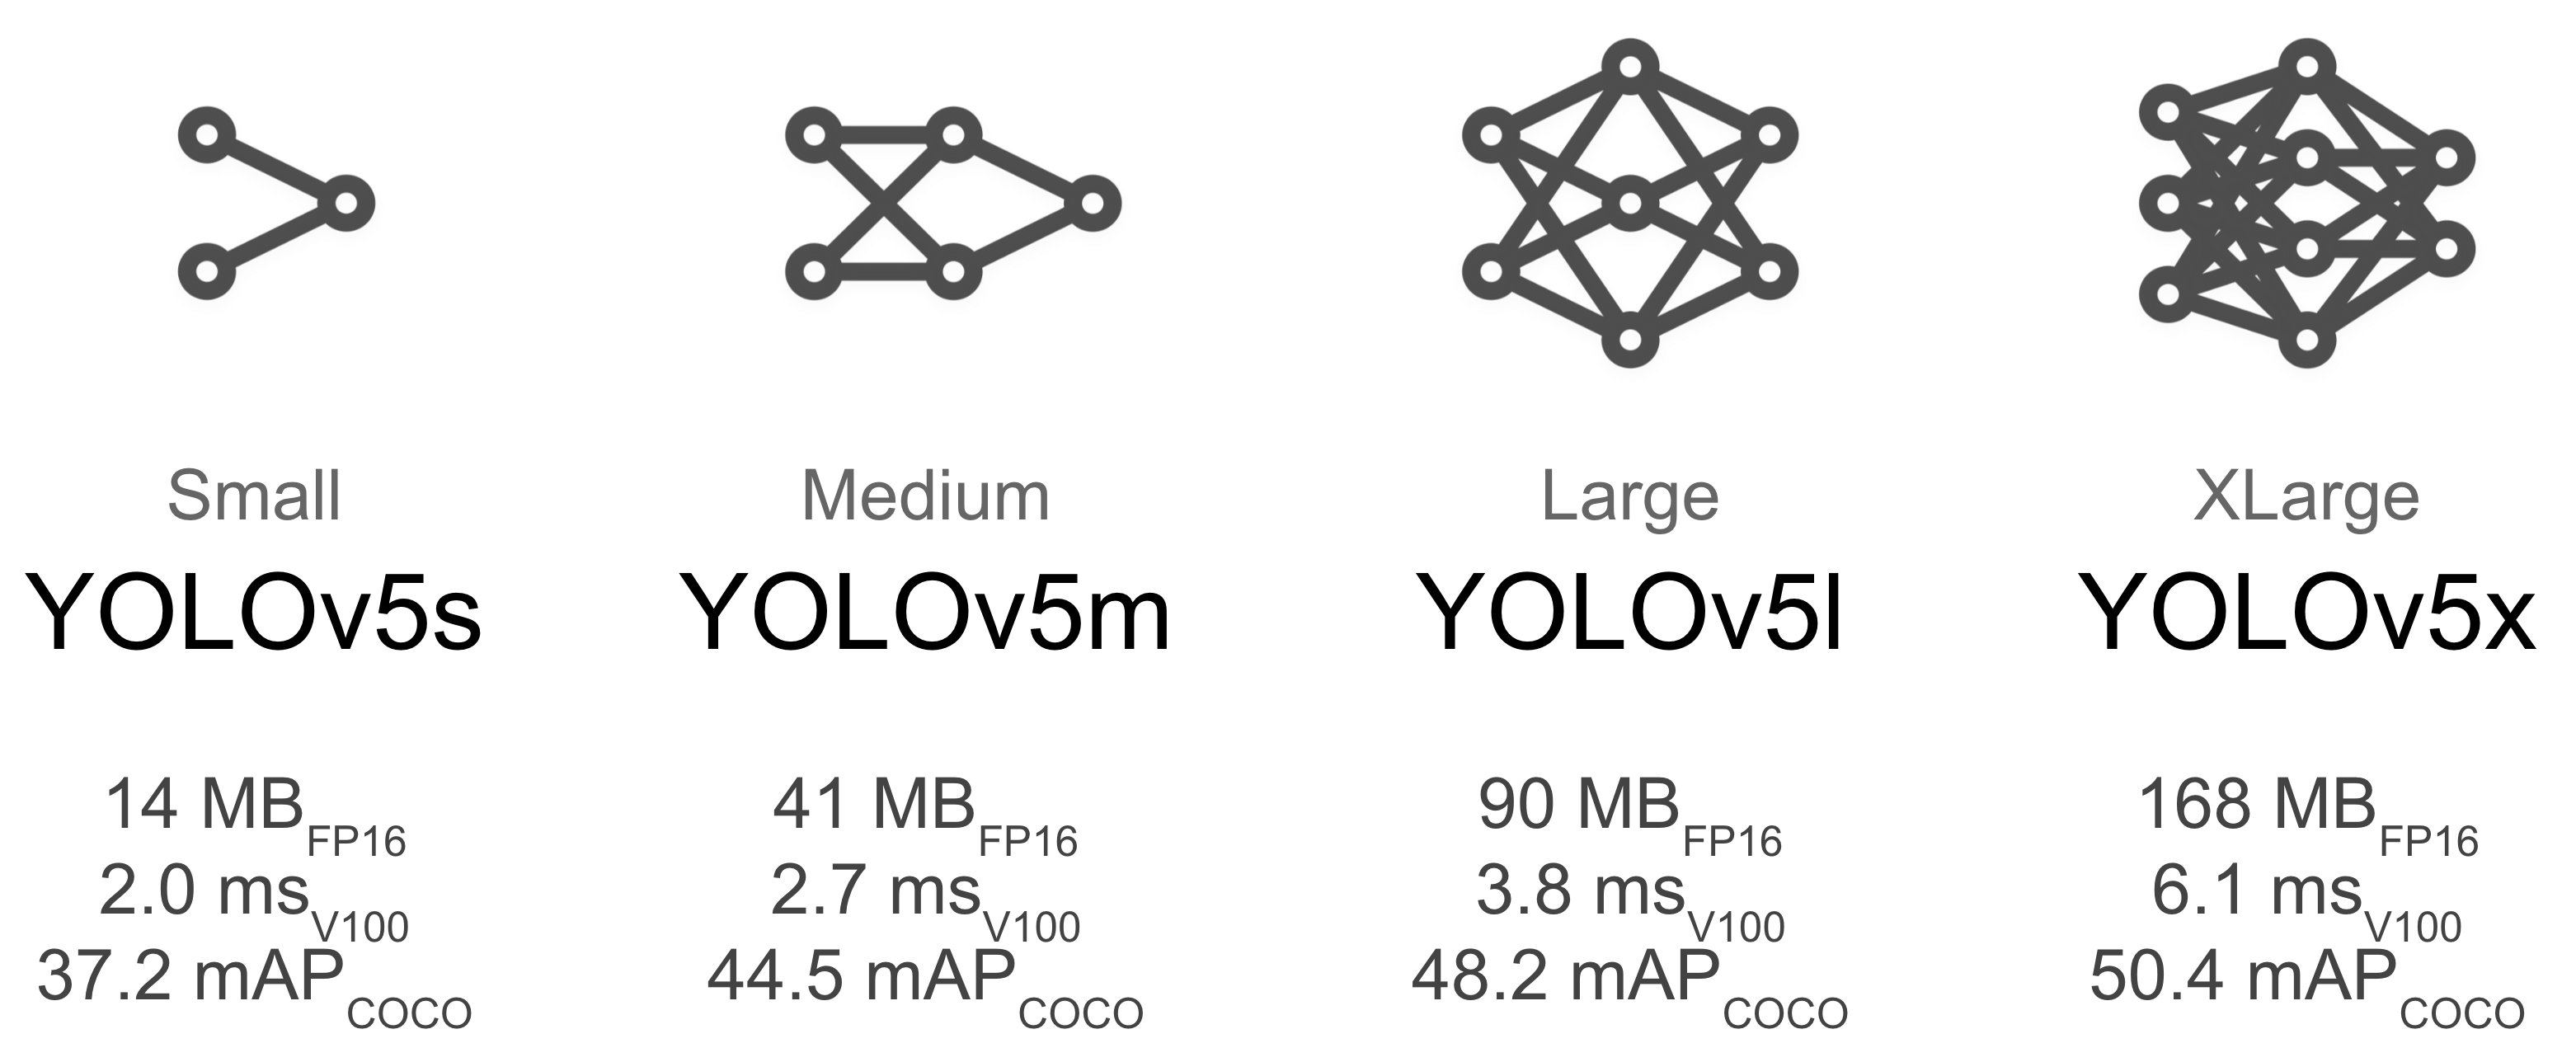
\includegraphics[width=1\linewidth]{images/yolov5.png}
            %        \end{figure}
            %    \end{column}
           % \end{columns}
            
            \begin{figure}[H]
                \centering
                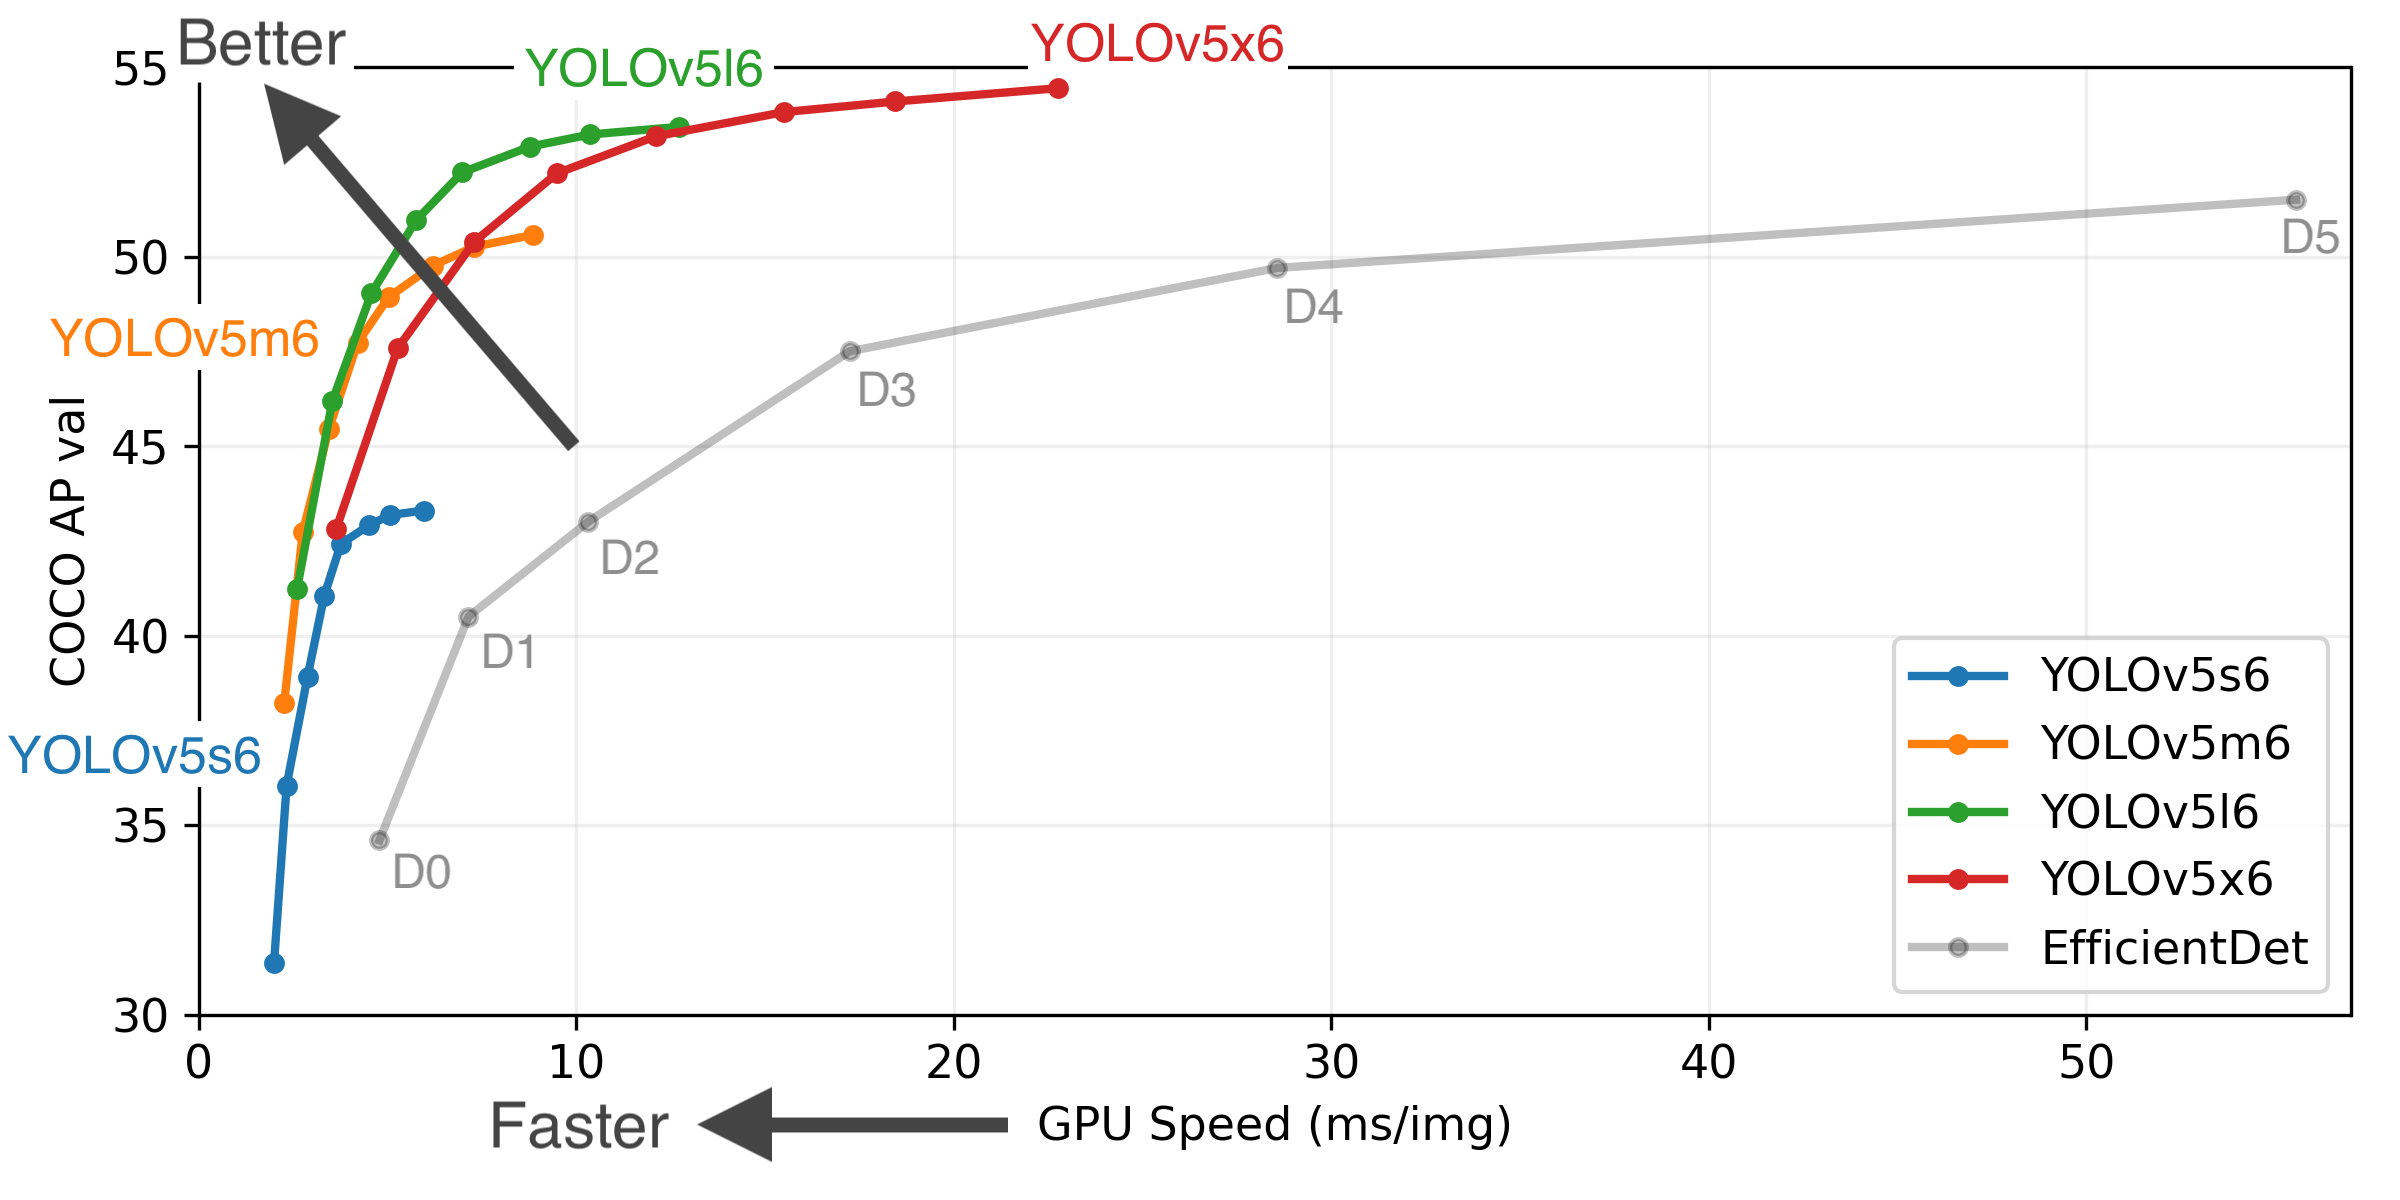
\includegraphics[width=0.9\linewidth]{images/modeleSpeedYolo.png}
                \caption*{Valeurs calculées avec une partie du dataset $COCO_{val2017}$ possédant +5000 images et 80 classes}
            \end{figure}
            
            \begin{block}{}
                \begin{itemize}
                    \setbeamertemplate{itemize item}[square]
                    \item Dataset de 75 images (25 bouchons, 25 tubes, 25 tubes colorés), prises grâce au Raspberry Pi, réparti :
                        \begin{itemize}
                            \item 70\% pour l'entrainement (51 images)
                            \item 30\% pour le test (24 images)
                        \end{itemize}
                    \item Modèle entraîné avec 1 batch et 100 epochs
                \end{itemize}
            \end{block}
            
            \begin{columns}
                \begin{column}{0.5\textwidth}
                    \begin{figure}[H]
                        \centering
                        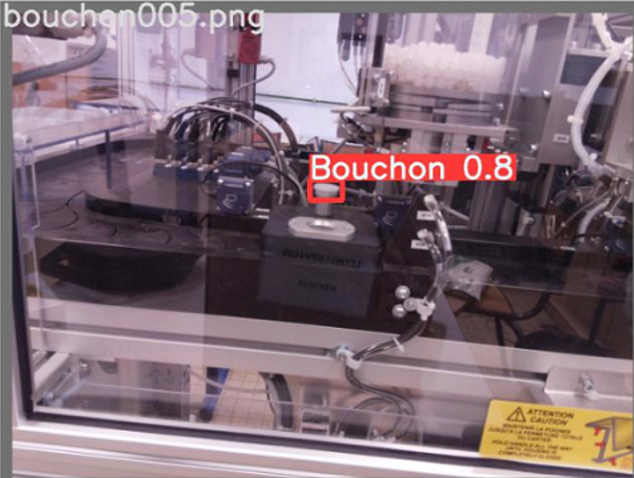
\includegraphics[width=0.9\linewidth]{images/pred_bouchon.png}
                    \end{figure}
                \end{column}\hfill
                \begin{column}{0.5\textwidth}
                    \begin{figure}[H]
                        \centering
                        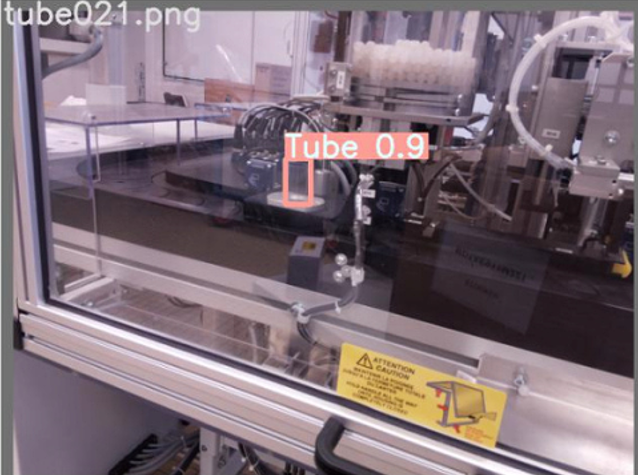
\includegraphics[width=0.9\linewidth]{images/pred_tube.png}
                    \end{figure}
                \end{column}
            \end{columns}
            
            \begin{figure}[H]
                \centering
                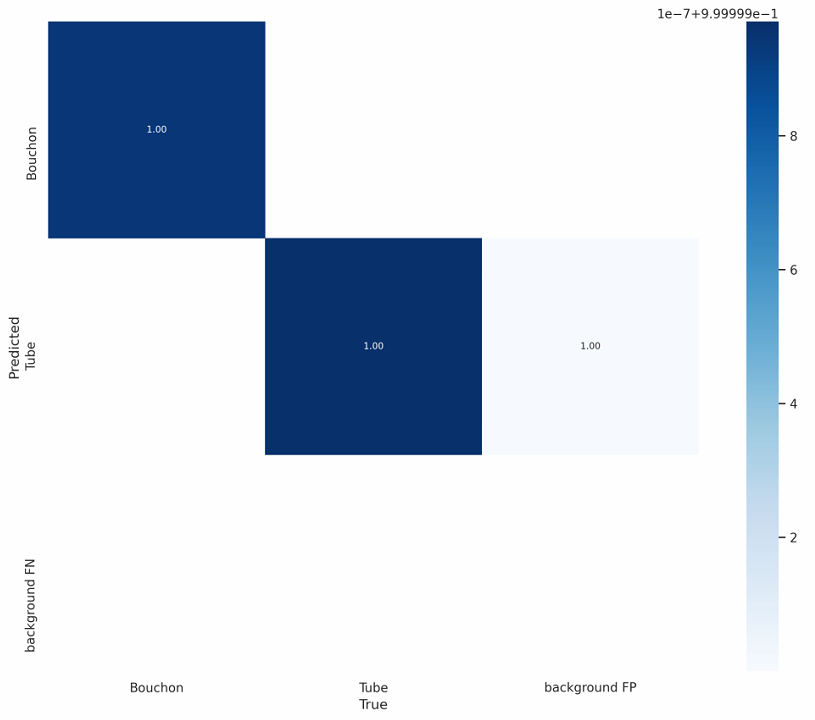
\includegraphics[width=.7\linewidth]{images/matriceConfusion.png}
            \end{figure}
            
            
        \end{frame}
%
% ---------------------------------------------------------------- %